% !TEX root=/home/tavant/these/manuscript/src/manuscript.tex

\section{PIC simulation results: Coche test-case}

In this sections, we present the results of the \ac{2D} \ac{PIC} simuations using the test-case of Coche, described in \cref{subsec-coche_description}; the parameters used are given in \vref{tab-parameters-coche}.
In this test-case, we use a permittivity scaling ($\epsilon_0^* = 80 \epsilon_0$) that allow us to observe the breathing mode.

The test-case of Coche has been simulated twice\string:
\begin{itemize}
  \item once without the radial losses, 
  \item once with the radial losses modeled, using $L_R = 2\,\centi\meter$.
\end{itemize}
 

\subsection{Coche test-case: results overview} \label{subsec-choche-overview}

In order to well resolve the breathing mode, the test-cases of Coche are simulated during 300\,\micro\second.
\Cref{fig-overview_coche_neEx} shows the axial and azimuthal distribution of the azimuthal electric field $E_{\theta}$ and the electron density $n_e$ at $t=236\,\micro\second$ is the case where no radial losses are modeled.
We see in both $E_{\theta}$ and $n_e$ the \ac{ECDI}, which wavelength is approximately $\lambda_{\theta} = 0.3\,\centi\meter$.
The results observed are similar to the one presented by \citet{coche2014}.
Hence, we expect that there is no error in the simulation.

\begin{figure}[hbt]
  \centering
  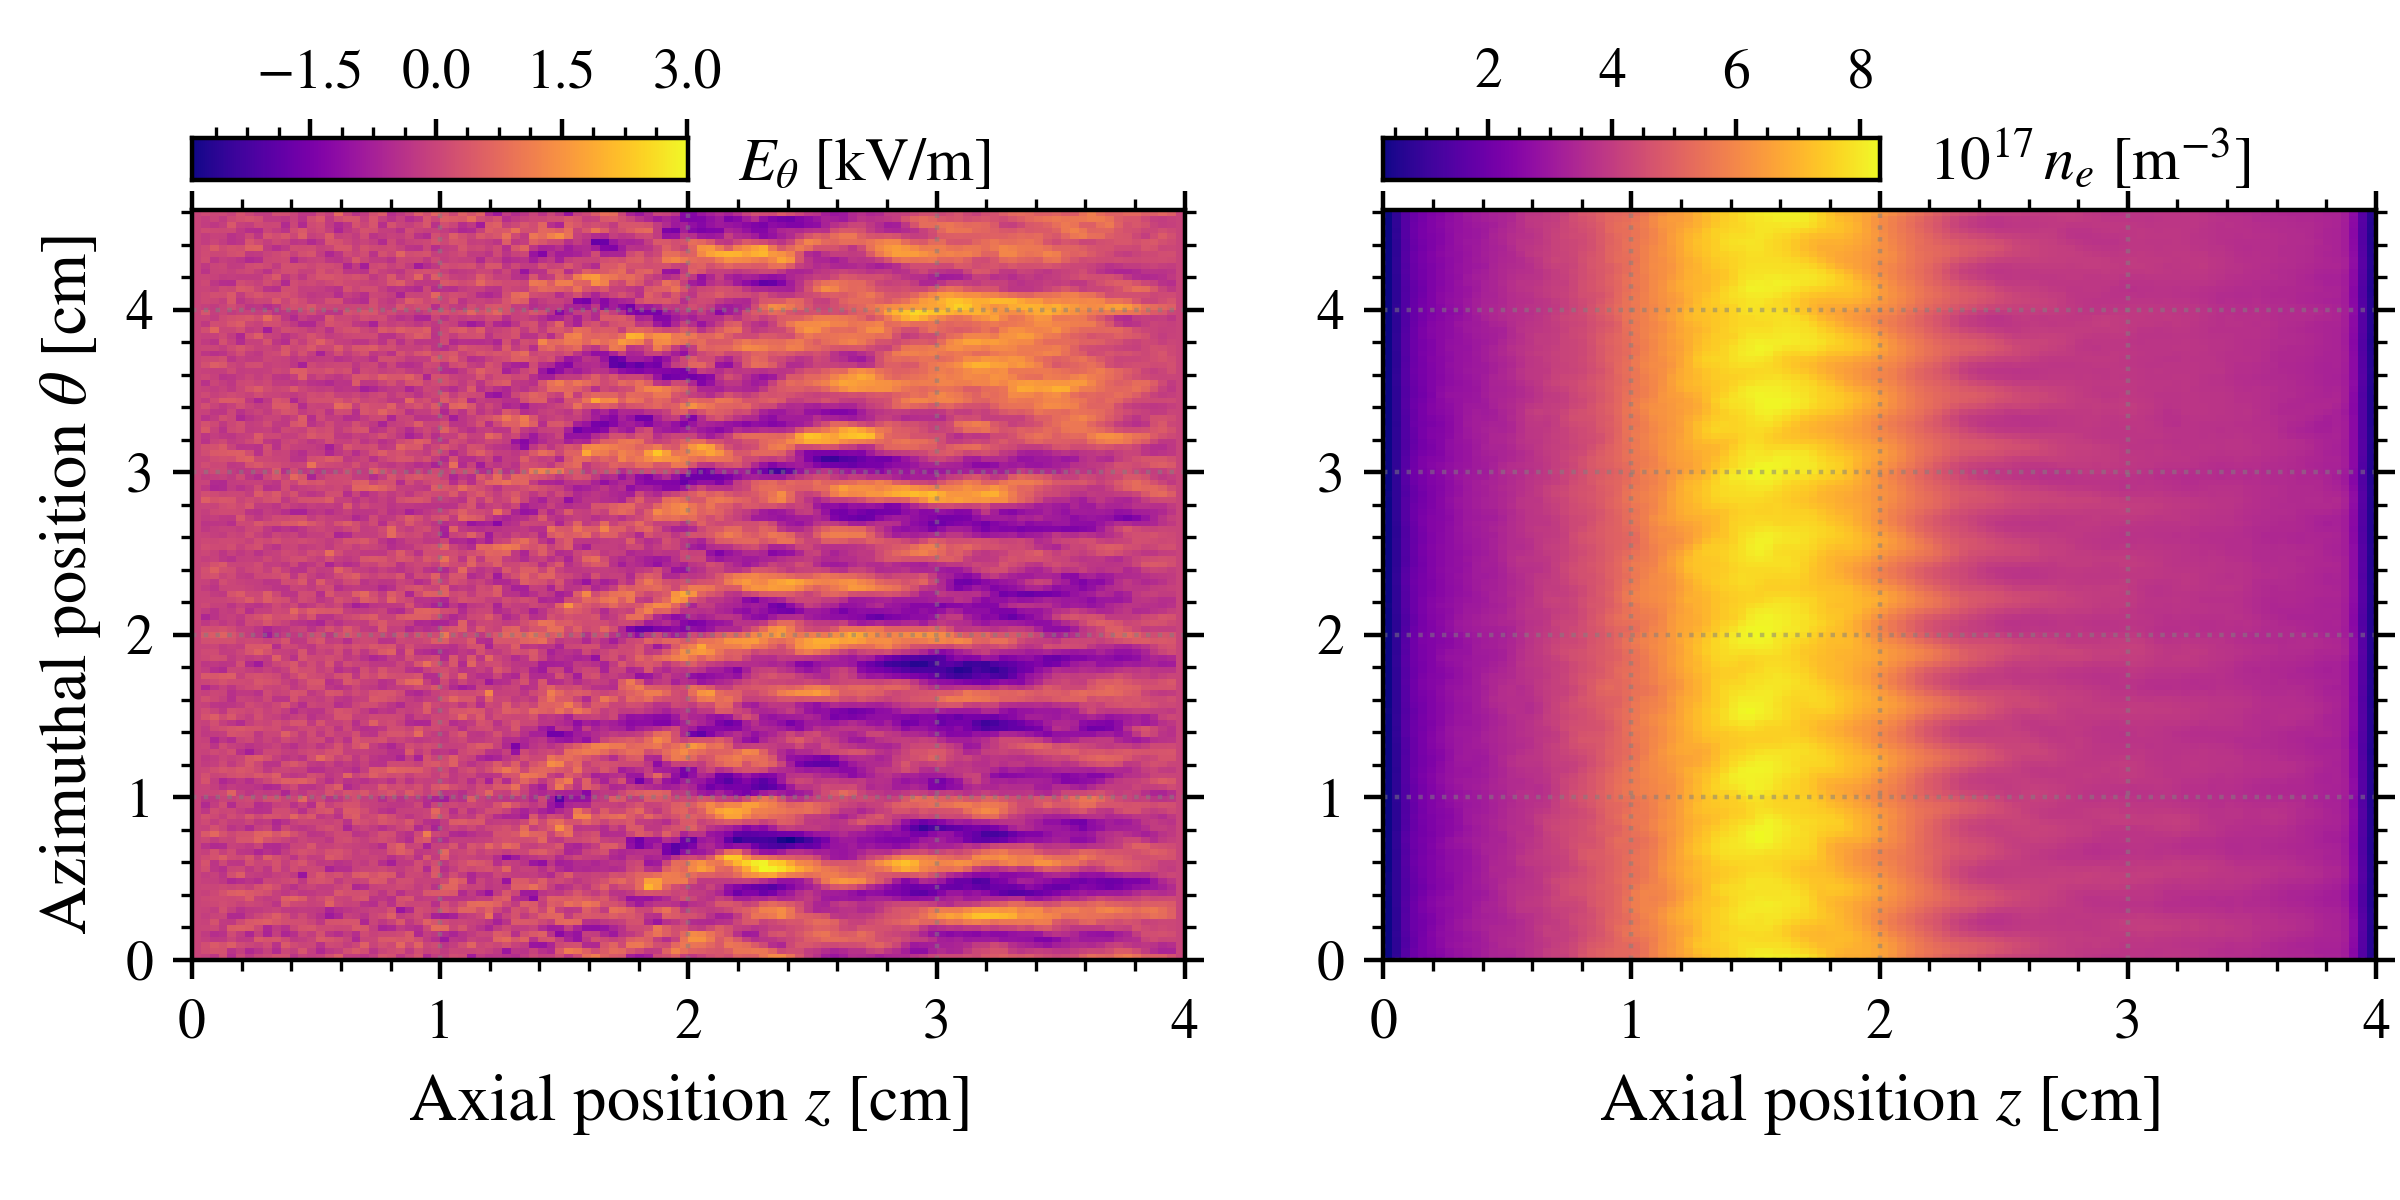
\includegraphics[width=0.9\textwidth]{Coche_example_t=236}
  \caption{ Axial-azimuthal distributions of (left) the azimuthal electric field $E_{\theta}$ and (right) the electron density $n_e$ at $t=236\,\micro\second$ for the test-case of Coche. } 
  \label{fig-overview_coche_neEx}
\end{figure}



\subsection{Coche test-case: Temporal evolution} \label{subsec-temp_coche}

\begin{figure}[hbt]
  \centering
  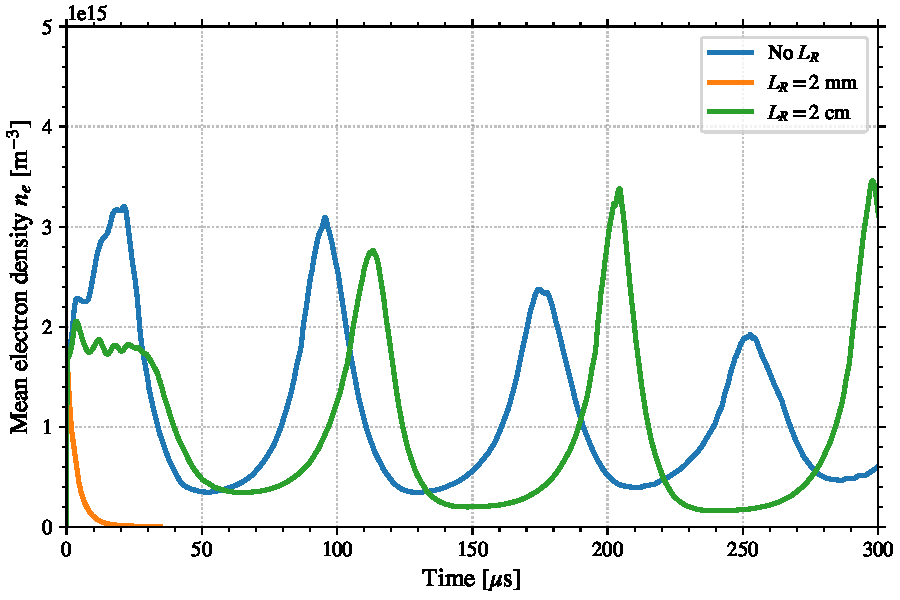
\includegraphics[width=\defaultwidth]{Coches_mean_ne}
  \caption{Temporal evolution of the average plasma density}
  \label{fig-coche_mean_ne}
\end{figure}

We  see in \Cref{fig-coche_mean_ne} the temporal evolution of the average plasma density in the \ac{PIC}  simulations.

We clearly observe the breathing mode on the mean plasma density.
In the case where no radial losses are modeled, the amplitude of the breathing mode decreases slightly.
On the other hand, its amplitude increases with the radial losses.
It could be due to the minimum density, that is lower with radial losses than without the losses.
Thus, the neutral density can increase to larger values, which induces a larger maximum density.

In \citet{hara2014}, the authors analyse the role of the electron energy balance in the breathing mode stability.
They showed that the electron power balance is important to describe the growth or the damping of the oscillation.


\subsection{Coche test-case: Axial profiles} \label{subsec-axial_coche}

  The axial profiles are averaged over the last breathing oscillation.
  This corresponds for the case without the radial losses model to averaging between $t=170\,\micro\second$ and $t=250\,\micro\second$.
  In the case with the radial losses, the average is done between $t=200\,\micro\second$ and $t=300\,\micro\second$.
  
  \begin{figure}[hbt]
    \centering
    \begin{tabular}{cc}
      \subfigure{Coches_mean_ne_profile}{a}{20,20} &
      \subfigure{Coches_mean_Ez_profile}{b}{20,15} \\
    \end{tabular}
    \caption{({\bf a}) Axial profile of the mean plasma density and  ({\bf b}) of the mean axial electric field obtained with and without the radial losses model  the simulation case of Coche. The variables are averaged  between $t=170\,\micro\second$ and $t=250\,\micro\second$ for the case without radial loss, and  between $t=200\,\micro\second$ and $t=300\,\micro\second$ for the case with the radial loss. }
    \label{fig-coche-axial-prof}
  \end{figure}
  
  \Cref{fig-coche-axial-prof} shows the axial profiles of the plasma density and the axial electric field averaged over an oscillation period.
  Both the density and the maximum of the electric field are smaller with the radial losses modeled.
  
  \Cref{fig-coche-axial-Te} shows the axial profiles of the electron temperature in the three directions averaged over an oscillation period.
  The axial and azimuthal present similar profiles as in the simulation case of Boeuf.
  Except that in this case, the maximum values are smaller and we have $\Te_z \sim \Te_{\theta}$.
  In addition, the electrons are less anisotropic, with a higher radial temperature.
  
  \begin{figure}[hbt]
    \centering
    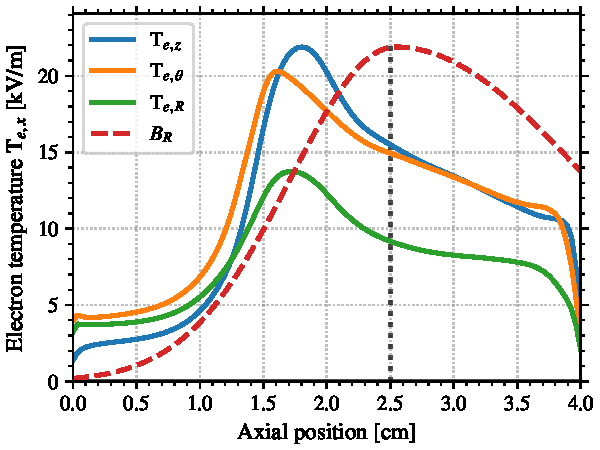
\includegraphics[width=0.6\textwidth]{Coches_mean_Tez_profile}
    \caption{ Axial profile of the mean electron temperature in the 3 directions for the case with radial losses. The variables are averaged  between $t=170\,\micro\second$ and $t=250\,\micro\second$ for the case without radial loss, and  between $t=200\,\micro\second$ and $t=300\,\micro\second$ for the case with the radial loss.}
    \label{fig-coche-axial-Te}
  \end{figure}
  
  \FloatBarrier

  